\section{The Symmetry Breaking Problem}
\label{cap:2}

A symmetric system can be defined as a system in which the processes are in an equivalent relationship, this means that if processes run the same code, it is possible to permute the processes without changing the behaviour of the system. One example of this state would be a ring in which there is no unique identifier for every process \cite{boldi1996symmetry}.

If we consider a message passing system in which exists an initial state of symmetry between all processes, there is an admissible synchronous execution for which the processes will continue in the same initial state. In this case, it is necessary a mechanism to break the symmetry, otherwise, the system cannot escape from the initial state.
%as shown in \cite{angluin1980local} by Angluin.

Symmetry breaking is one of the most extensively studied problems in distributed computing. The fundamental symmetry breaking problems on graph include the maximal matching, vertex colouring, ruling sets and \textit{MIS}. The last one can be considered as the central problem because all the others can be reduced to it, as shown in  \cite{linial1992locality}.Two problems related to the maximal independent set are studied in the literature. Finding the \textit{MIS} of a general graph and listing all the \textit{MISs} in a given graph. In the next section, a formal definition of the maximal independent set is given. A  discussion on the sequential approach vs the distributed approach is presented with the theoretical analysis on time complexity and message complexity in the case of the distributed approach.     

\subsection{Maximal Independent Set}

\theoremstyle{definition}
\begin{definition}

Given an undirected graph $G = (V,E)$, a Maximal Independent Set \textbf{MIS} is a set of vertices $S \subseteq V$ if it satisfied the following properties:   

\begin{enumerate}
  \item the set MIS is an independent set meaning that no two vertices $v,u \in S$ are adjacent,
  \item the set S is maximal, with regard to independence, meaning that for each vertex $v \notin MIS$, there exists a neighbour $u$ of $v$ such that $u \in MIS$.
\end{enumerate}

\end{definition}

Figure \ref{fig:graph1} shows an example of undirected an graph $G$ with 8 vertices and 14 edges. There are two \textit{MIS} in this example, showing that it is possible to find more that one solution for the same instance of $G$. The green nodes are part of the \textit{MIS}, in the first \textit{MIS} the number of nodes is 2 and 4 in the second solution. Note that no common edges exist between green vertices and every vertex that it is not part of the \textit{MIS} has a neighbour in it, satisfying the conditions set out above.
 
\begin{figure}[ht]
\centering
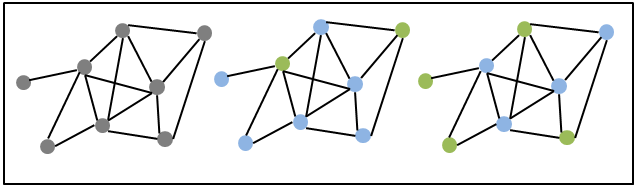
\includegraphics[width=1 \linewidth, height=5cm]{mis-example.PNG} 
\caption{Example of two Maximal Independent Set of a general graph}
\label{fig:graph1}
\end{figure}



The algorithm \ref{algorithm:secuential-mis} describes the general sequential algorithm to find the maximal independent set of a general graph. The time complexity is $O(N)$ since in the worst case, the algorithm has to check every vertex. Another approach to improve this time is desirable. In the next section, two distributed algorithms to find the \textit{MIS} are presented.



\begin{algorithm}
 \caption{Sequential Maximal Independent Set}
 \label{algorithm:secuential-mis} 

\SetAlgoNoLine
\KwResult{MIS Maximal Independent Set}
\KwData{ $G(V,E)$ Graph}
    \While {$V$ is not empty}{
        Choose a vertex $v \in V$
            Add $v$ to the set MIS\;
            Remove from $V$ the vertex $v$ and all its neighbours\;
        }
    
 
\end{algorithm}
 
 
\subsection{Distributed Maximal Independent Set}

A logarithmic lower bound is in general acceptable to consider a problem to be optimally solved. The difficulty to find it in sequential algorithms motivated the proposal of distributed algorithms. Deterministic and randomised algorithms are the approaches to solve problems in distributed computing.  Applying randomisation techniques on algorithms is a powerful and efficient technique to solve problems that may take longer time in a deterministic algorithm.

In 1986, an efficient distributed algorithm was proposed independently by Luby \cite{luby1986simple} and Alon \textit{et al.} \cite{alon1986fast}. Both algorithms are randomised and the expected termination time is $O(log N)$ rounds. It is worth to mention that all algorithms exposed below run in the synchronous model.  

The algorithm\ref{algorithm:luby-mis} describes the original Luby's algorithm. Prove the correctness of this algorithm is very simple. If a vertex joins the \textit{MIS}, in a round $r$, no other neighbour join the set in $r$ or in any other $r\prime$. The algorithm at the end produces a \textit{MIS} because the vertices with the highest degree will decide to enter the \textit{MIS} in each round until all vertices become inactive.

\begin{definition}

An algorithm terminates with high probability (w.h.p.) within $O(t)$ time if it does so with probability at least $1-\frac{1}{n^c}$ for any choice of $c\geq 1$.

\end{definition}

%  Message complexity depends on the number of processes which are active in each phase and its denoted by $O(m)$ in \cite{luby1986simple}. With high probability $\frac{1-1}{n}$, the Luby's algorithm finishes  $4\log N$ round. 

% \theoremstyle{theorem}
\begin{theorem}

Algorithm \ref{algorithm:luby-mis} computes a maximal independent set for any graph  in $O(\log n)$  rounds with high probability.

\end{theorem}


\begin{algorithm}
 \caption{Luby's Algorithm, code for each process $p_i$ $i = 1$ to $N$}
 \label{algorithm:luby-mis} 

\SetAlgoNoLine
\KwResult{MIS Maximal Independent Set}
\KwData{ $G(V,E)$ Graph}
    \While {V is not empty}{
        Choose a random set of vertices $S ⊆ V$, by selecting each vertex $v$ independently with probability $1/(2d(v))$, where d is the degree of $v$\;
        For every edge $e \in E$, if both its endpoints are in the random set $S$, then remove from $S$ the endpoint whose degree is lower. Break ties arbitrarily, e.g. using a lexicographic order on the vertex names\;
        Add the set $S$ to $MIS$\;
        Remove from $V$ the set $S$ and all the neighbours of vertices in $S$\;
        }
\end{algorithm} 



The algorithm \ref{algorithm:main-mis} is another randomised distributed algorithm and was proposed by Yves \cite{yves2009optimal}. This algorithm is used for the simulations in this project and it is a variation of Luby's algorithm. The rounds can be split into 2 phases for simplicity. In each phase, each process chooses a random value, send it to its neighbours and wait to receive the value from all its neighbours. If the process has the maximum value, the join the \textit{MIS}. In the second phase, if the $p_i$ decided to join the $MIS$, then notified its neighbours that $p_i$ is part of the \textit{MIS}. If $p_j$ receives the last notification message from $p_i$, then $p_j$ decide not to join the \textit{MIS}. At the end of this phase, every process that made a decision about joining or not the \textit{MIS} become inactive for the next rounds.

\begin{algorithm}
 \caption{MIS Algorithm, code for each process $p_i$ from $i = 1$ to $N$}
 \label{algorithm:main-mis} 

\SetAlgoNoLine
\KwResult{MIS Maximal Independent Set}
\KwData{ $G(V,E)$ Graph}
    \While {V is not empty}{
        $p_i$ select a random number $r(v)$ between [0,1] and sends to its neighbours\;
        If $r(v) < r(w)$ for all neighbours $w \in N(v)$ of $p_i$, remove myself from $V$ and enter to the MIS \newline
        Inform my neighbours that I am a MIS member and terminate\;
        If $p_i$ heard that my neighbour $p_j$ is in the MIS, remove myself from the $V$ and terminate\;
        }
\end{algorithm}

% Lemma 7.14 (Edge Removal). In a single phase, we remove at least half of
% the edges in expectation.

The correctness is very intuitive and similar to the Luby's algorithm. In one phase, one process $p_i$ joins the \textit{MIS} only if it has the largest value among its neighbours. At the end of that phase, all the neighbourhood of $p_i$ become inactive, including $p_i$ and there is no neighbour of $p_i$ in the \textit{MIS}. This set is maximal because at least one vertex (with the global smallest value) will enter into the \textit{MIS} per round, hence there is a progress in each round. If at some round, a vertex has no neighbours, it automatically joins the set and become inactive. This sequence continues in the following rounds until every process becomes inactive.

% \theoremstyle{theorem}
\begin{theorem}

Algorithm \ref{algorithm:main-mis} computes a maximal independent set for any graph in $O(\log n)$ rounds with high probability.

\end{theorem}


 Until now, these two algorithms are faster than the best deterministic algorithms for general graphs. There have been some improvements for special cases, for instance, \cite{panconesi1996complexity} proposed a $O(\Delta + log^* N)$ algorithm for specific graphs, however, the original algorithms are still faster when the running time is expressed as a function of $N$ and for any type of graph.
 
 In a round when a vertex join the \textit{MIS} all the edges of $v$ and the edges of any neighbour of $v$ are removed from $E$. In general, this number is much grater that the degree of $v$. So there is a high probability that the topology decreases very fast. Indeed, this is the mechanism to demonstrate the lower bound of $O(\log N)$. In the section \ref{chap:6} (Evaluation of results), this supposition is tested experimentally. 
 

% . This algorithm operates in synchronous rounds. In line 2, every process select a random number to in order to break the symmetry with its neighbours, line 3 makes sure that if a vertex v join the MIS, no other neighbour of v join the MIS at the same time, this is true because the execution  occurs in rounds. the line 4 makes sure that any vertex that has a neighbour in the MIS, join the MIS at any point. 


\newpage